% !TeX document-id = {31cec06c-209e-42c6-b48d-393b1a0af1d2}
% !TeX TS-program = xelatex
% !BIB TS-program = biber
% !TeX encoding = UTF-8
% !TeX spellcheck = en_US
% !TeX root = seminar_presentation__intelligent_industrial_robots.tex


%% LaTeX-Beamer template for KIT design
%% by Erik Burger, Christian Hammer
%% title picture by Klaus Krogmann
%%
%% version 2.1
%%
%% mostly compatible to KIT corporate design v2.0
%% http://intranet.kit.edu/gestaltungsrichtlinien.php
%%
%% Problems, bugs and comments to
%% burger@kit.edu

\documentclass[18pt]{beamer}

\usepackage[utf8]{inputenc}

%% SLIDE FORMAT

% use 'beamerthemekit' for standard 4:3 ratio
% for widescreen slides (16:9), use 'beamerthemekitwide'
% for widescreen slide without sidebar use 'beamerthemekitwidenosidebar'

%\usepackage{templates/beamerthemekit}
%\usepackage{templates/beamerthemekitwide}
\usepackage{templates/beamerthemekitwidenosidebar}

% use this to disable the latex beamer navigation symbols
%\beamertemplatenavigationsymbolsempty


%% TITLE PICTURE

% if a custom picture is to be used on the title page, copy it into the 'logos'
% directory, in the line below, replace 'mypicture' with the 
% filename (without extension) and uncomment the following line
% (picture proportions: 63 : 20 for standard, 169 : 40 for wide
% *.eps format if you use latex+dvips+ps2pdf, 
% *.jpg/*.png/*.pdf if you use pdflatex)

\titleimage{plc_logo}

%% TITLE LOGO

% for a custom logo on the front page, copy your file into the 'logos'
% directory, insert the filename in the line below and uncomment it

\titlelogo{iar_iirob}

% (*.eps format if you use latex+dvips+ps2pdf,
% *.jpg/*.png/*.pdf if you use pdflatex)

%% TikZ INTEGRATION

% use these packages for PCM symbols and UML classes
\usepackage{templates/tikzkit}
\usepackage{templates/tikzuml}

\usepackage{tabularx}
\usepackage{multirow}
\usepackage{multicol}
\usepackage{booktabs}

\usepackage{glossaries}
\usepackage{acronym}
\usepackage{listings}

% the presentation starts here

\title[Automated Programming of Programmable Logic Controllers]{Seminar Intelligent Industrial Robots}
\subtitle{Automated Programming of Programmable Logic Controllers}
\author{David Oberacker}

\institute{
	Institute for Anthropomatics and Robotics - Intelligent Process Automation and Robotics Lab (IAR-IPR)
}

% Bibliography

\usepackage[citestyle=authoryear,bibstyle=numeric,hyperref,backend=biber]{biblatex}
\addbibresource{presentation.bib}
\bibhang1em

\newacronym{acn:PLC}{PLC}{Programmable Logic Controller}

\makeglossaries

\begin{document}

% change the following line to "ngerman" for German style date and logos
\selectlanguage{english}

%title page
\begin{frame}
\titlepage
\end{frame}

%\begin{frame}{Introduction}
%    \begin{figure}
%        \centering
%        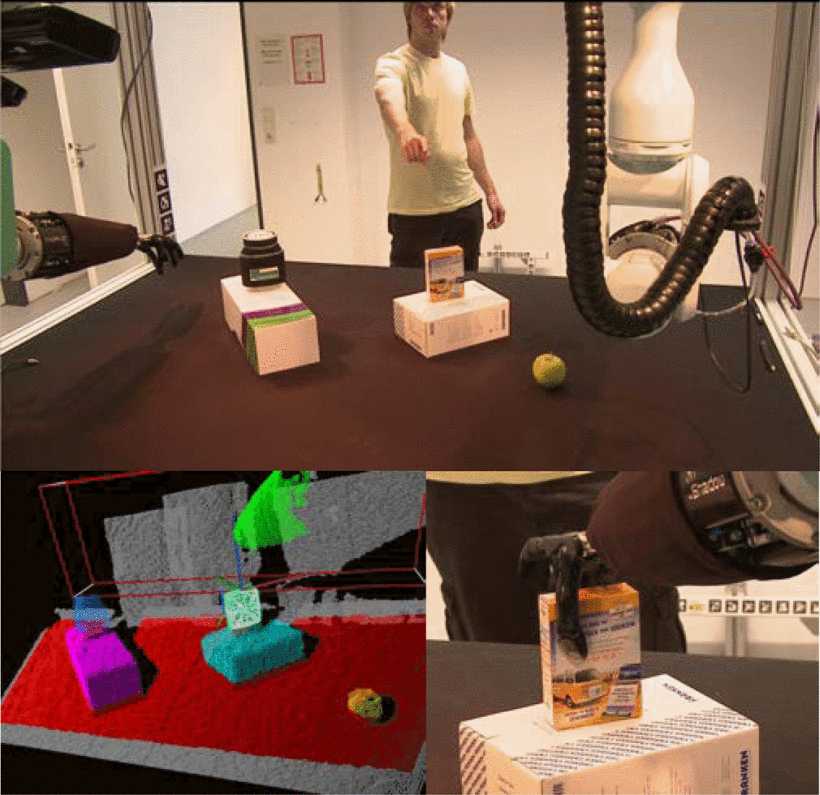
\includegraphics[height=0.7\textheight]{figures/3d_semantic_grasping.png}
%    \end{figure}
%\footcitetext{6385692}
%\end{frame}

%table of contents
\begin{frame}{Outline}
\tableofcontents
\end{frame}

\section{Introduction}

\begin{frame}{Introduction}
    
    \begin{itemize}
        \item Automation is a important factor in todays industry.
        \item With Industry 4.0 automation systems have to get more flexible.
        \item Common controller in automation are~\acrfull{acn:PLC}.
        \item They are programmed in a static and non-flexible manner.
    \end{itemize}
    $\Rightarrow $ Are there ways to program a~\acrshort{acn:PLC} in a more flexible way ?
    
\end{frame}

\section{Programmable logic controller}

\begin{frame}{Programmable Logic Controller}
\begin{columns}
    \begin{column}{0.5\textwidth}
        \begin{itemize}
            \item Specialized industrial computers.
            \item Fixed~\textbf{cycle based} execution semantic:
            \begin{enumerate}
                \item Copy~\textbf{input} variables values from the physical interfaces to the RAM.
                \item \textbf{Execution} of the~\textbf{user program}.
                \item Copy~\textbf{output} variable values from the RAM to the physical interfaces.
            \end{enumerate}
            \item Programmed via the languages defined in the IEC 61131-3 standard.
        \end{itemize}
    \end{column}
    \begin{column}{0.5\textwidth}
        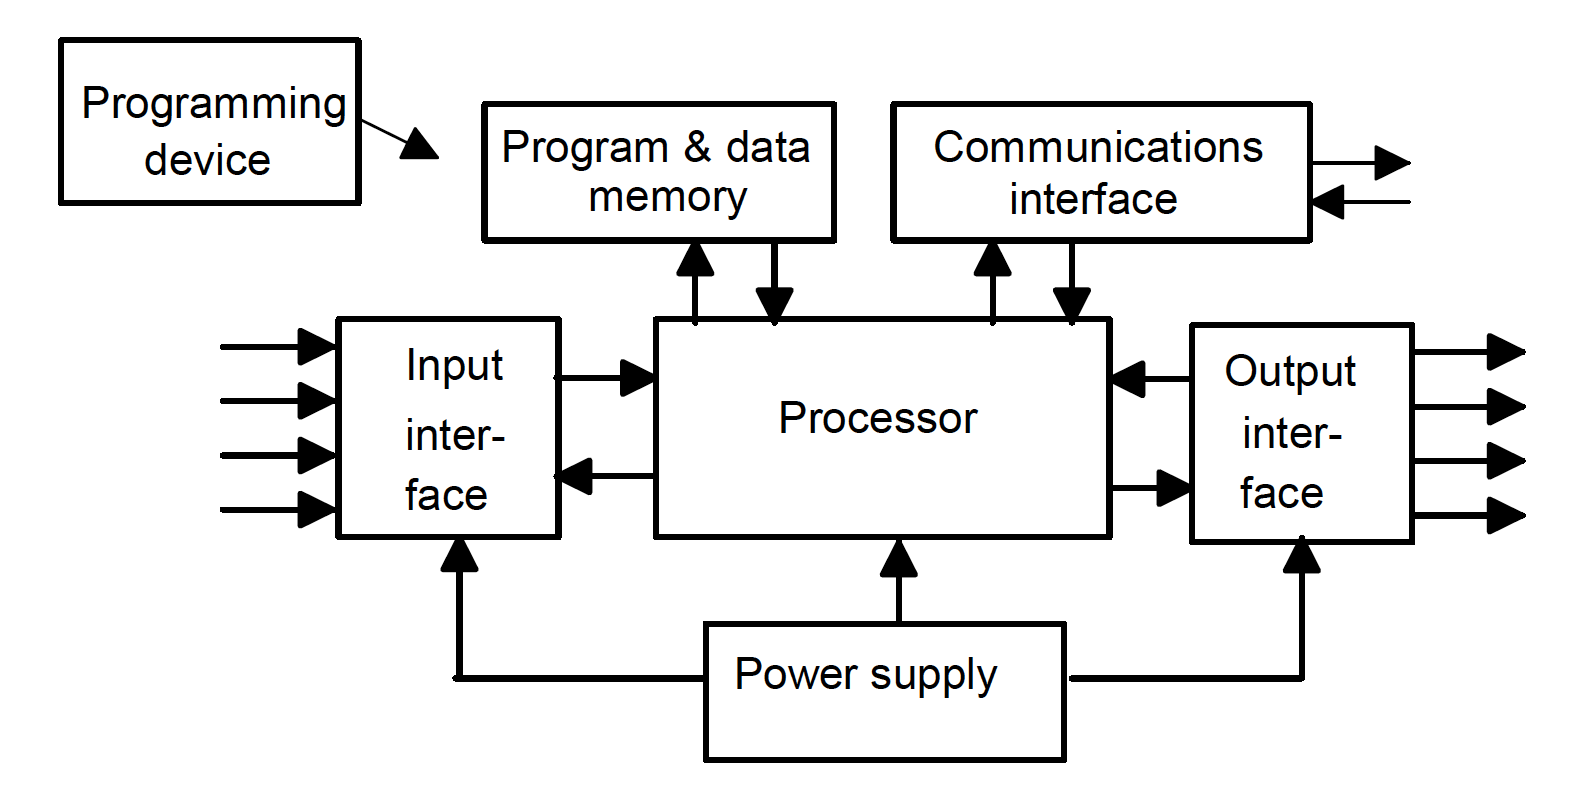
\includegraphics[width=\textwidth]{figures/PLC_Architecture.png}
        {\footnotesize Source:~\cite{BOLTON200653}}
    \end{column}
\end{columns}
\end{frame}

\subsection{IEC 61131-3 Languages}

\begin{frame}{Ladder Diagram}
\begin{columns}
	\begin{column}{0.5\textwidth}
		\begin{itemize}
            \item Graphical programming language.
            \item Historical importance.
			\item Similar to electrical relay diagrams.
			\item The named contacts are inputs, outputs and state variables.
			\item Can be combined with different operators (e.g. Not, $ >$, etc.).
		\end{itemize}
	\end{column}
	\begin{column}{0.5\textwidth}
		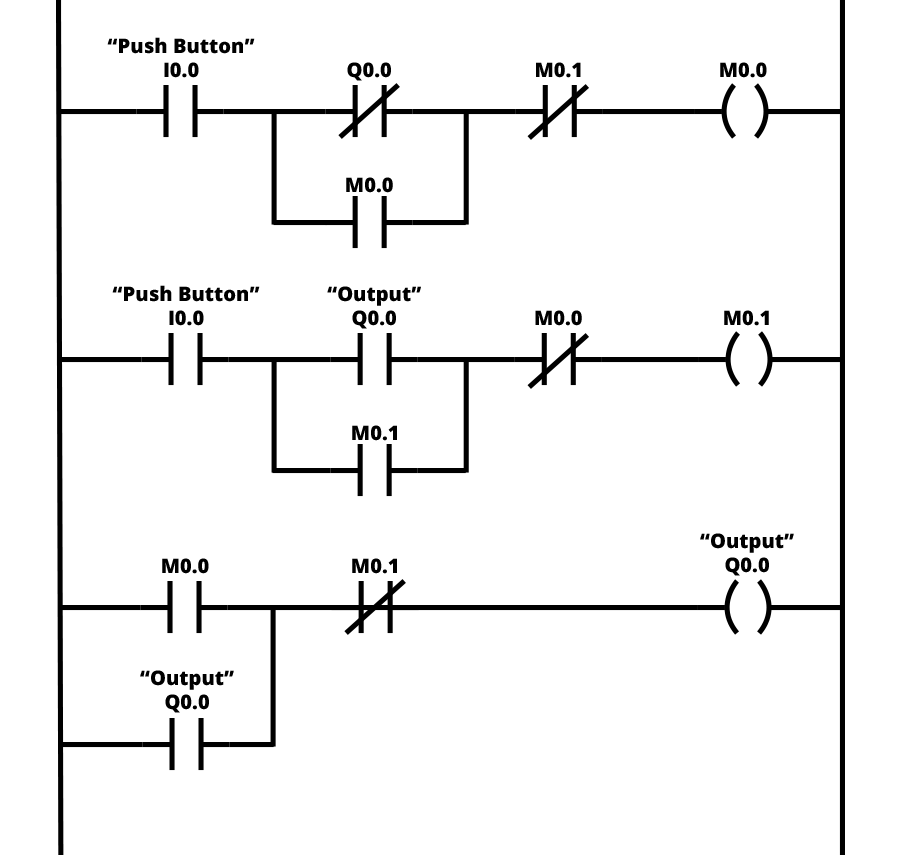
\includegraphics[width=0.8\textwidth]{figures/ld.png}
       {\footnotesize  Source:~\url{https://www.plcacademy.com/ladder-logic-examples/}}
	\end{column}
\end{columns}
\end{frame}

\begin{frame}[fragile]{Structured Text}
    \begin{columns}
        \begin{column}{0.5\textwidth}
           \begin{itemize}
               \item Textual programming language.
               \item Syntax is similar to PASCAL.
               \item Allows for more complex control flows.
               \item Currently the most used IEC 61131-3 language.
           \end{itemize}
        \end{column}
        \begin{column}{0.5\textwidth}
            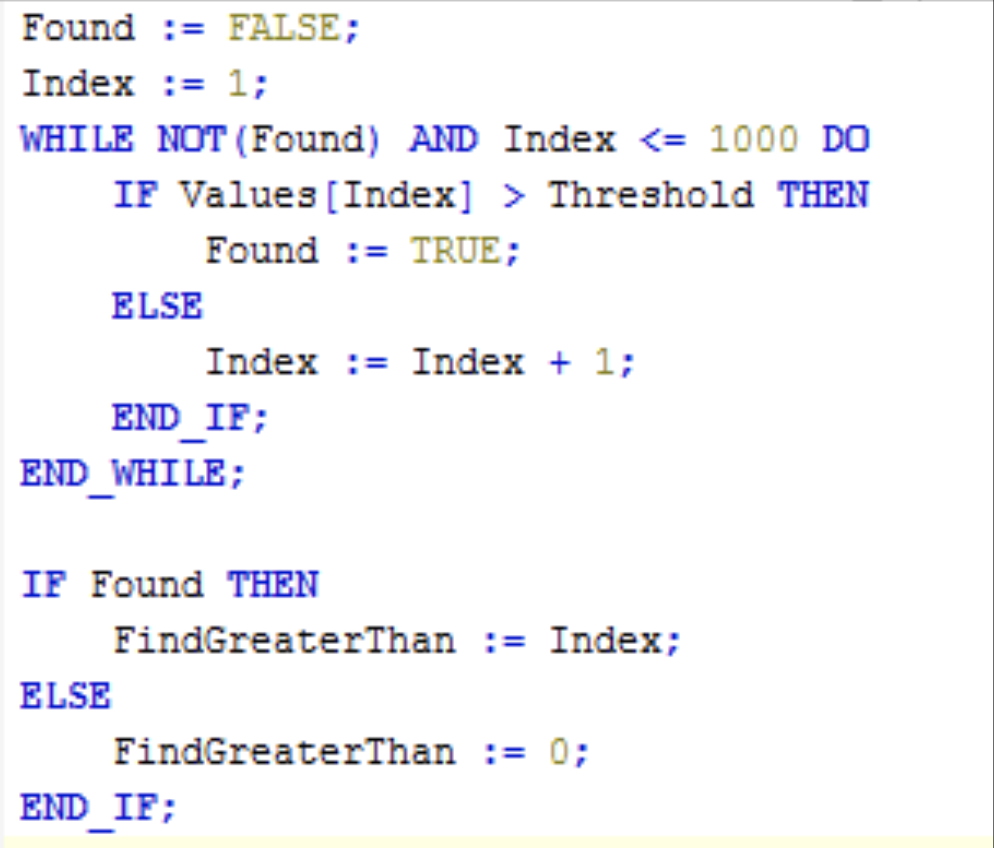
\includegraphics[width=0.8\textwidth]{./figures/st.png}
            {\footnotesize Source:~\url{http://www.contactandcoil.com/twincat-3-tutorial/structured-text/}}
        \end{column}
\end{columns}
\end{frame}

\section{Automated programming of PLCs}

\begin{frame}{Datasets}
\begin{itemize}
    \item Common Objects in Context (COCO)
    \begin{itemize}
        \item 115 000 annotated images.
        \item Indoor and outdoor scenes.
        \item 80 foreground object classes.
    \end{itemize}
    \item Falling Things Dataset (FAT)
    \begin{itemize}
        \item 60 000 annotated images.
        \item Synthetic dataset.
        \item Objects failing through synthetic backgrounds.
    \end{itemize}
    \item YCB Video Dataset (YCB)
    \begin{itemize}
        \item 12 000 annotated images.
        \item Video frames from a camera pan around objects.
        \item Same objects as in the FAT dataset.
    \end{itemize}
\end{itemize}
\end{frame}

\subsection{C/C++-based programming}

\begin{frame}{Datasets}
\begin{itemize}
	\item Common Objects in Context (COCO)
	\begin{itemize}
		\item 115 000 annotated images.
		\item Indoor and outdoor scenes.
		\item 80 foreground object classes.
	\end{itemize}
	\item Falling Things Dataset (FAT)
	\begin{itemize}
		\item 60 000 annotated images.
		\item Synthetic dataset.
		\item Objects failing through synthetic backgrounds.
	\end{itemize}
	\item YCB Video Dataset (YCB)
	\begin{itemize}
		\item 12 000 annotated images.
		\item Video frames from a camera pan around objects.
		\item Same objects as in the FAT dataset.
	\end{itemize}
\end{itemize}
\end{frame}

\subsection{Formal description based}

\begin{frame}{Linear Temporal Logic}
\begin{itemize}
	\item Common Objects in Context (COCO)
	\begin{itemize}
		\item 115 000 annotated images.
		\item Indoor and outdoor scenes.
		\item 80 foreground object classes.
	\end{itemize}
	\item Falling Things Dataset (FAT)
	\begin{itemize}
		\item 60 000 annotated images.
		\item Synthetic dataset.
		\item Objects failing through synthetic backgrounds.
	\end{itemize}
	\item YCB Video Dataset (YCB)
	\begin{itemize}
		\item 12 000 annotated images.
		\item Video frames from a camera pan around objects.
		\item Same objects as in the FAT dataset.
	\end{itemize}
\end{itemize}
\end{frame}

\begin{frame}{UML / SysML}
\begin{itemize}
	\item Common Objects in Context (COCO)
	\begin{itemize}
		\item 115 000 annotated images.
		\item Indoor and outdoor scenes.
		\item 80 foreground object classes.
	\end{itemize}
	\item Falling Things Dataset (FAT)
	\begin{itemize}
		\item 60 000 annotated images.
		\item Synthetic dataset.
		\item Objects failing through synthetic backgrounds.
	\end{itemize}
	\item YCB Video Dataset (YCB)
	\begin{itemize}
		\item 12 000 annotated images.
		\item Video frames from a camera pan around objects.
		\item Same objects as in the FAT dataset.
	\end{itemize}
\end{itemize}
\end{frame}

\begin{frame}{Simulink}
\begin{itemize}
	\item Common Objects in Context (COCO)
	\begin{itemize}
		\item 115 000 annotated images.
		\item Indoor and outdoor scenes.
		\item 80 foreground object classes.
	\end{itemize}
	\item Falling Things Dataset (FAT)
	\begin{itemize}
		\item 60 000 annotated images.
		\item Synthetic dataset.
		\item Objects failing through synthetic backgrounds.
	\end{itemize}
	\item YCB Video Dataset (YCB)
	\begin{itemize}
		\item 12 000 annotated images.
		\item Video frames from a camera pan around objects.
		\item Same objects as in the FAT dataset.
	\end{itemize}
\end{itemize}
\end{frame}

\begin{frame}{plcSpecif}
\begin{itemize}
	\item Common Objects in Context (COCO)
	\begin{itemize}
		\item 115 000 annotated images.
		\item Indoor and outdoor scenes.
		\item 80 foreground object classes.
	\end{itemize}
	\item Falling Things Dataset (FAT)
	\begin{itemize}
		\item 60 000 annotated images.
		\item Synthetic dataset.
		\item Objects failing through synthetic backgrounds.
	\end{itemize}
	\item YCB Video Dataset (YCB)
	\begin{itemize}
		\item 12 000 annotated images.
		\item Video frames from a camera pan around objects.
		\item Same objects as in the FAT dataset.
	\end{itemize}
\end{itemize}
\end{frame}

\begin{frame}{GRAFCET}
\begin{itemize}
	\item Common Objects in Context (COCO)
	\begin{itemize}
		\item 115 000 annotated images.
		\item Indoor and outdoor scenes.
		\item 80 foreground object classes.
	\end{itemize}
	\item Falling Things Dataset (FAT)
	\begin{itemize}
		\item 60 000 annotated images.
		\item Synthetic dataset.
		\item Objects failing through synthetic backgrounds.
	\end{itemize}
	\item YCB Video Dataset (YCB)
	\begin{itemize}
		\item 12 000 annotated images.
		\item Video frames from a camera pan around objects.
		\item Same objects as in the FAT dataset.
	\end{itemize}
\end{itemize}
\end{frame}

\section{Risks of automated programming}

\begin{frame}{Transformation function correctness}

\begin{block}{Transformation function correctness}
	\begin{itemize}
		\item Processing time is strongly bound to the architecture.
		\item Optimizing the processing times is a important topic for modern architectures.
	\end{itemize}
\end{block}
\end{frame}

\begin{frame}{Runtime guarantees}

\begin{block}{Runtime guarantees}
	\begin{itemize}
		\item Processing time is strongly bound to the architecture.
		\item Optimizing the processing times is a important topic for modern architectures.
	\end{itemize}
\end{block}
\end{frame}

\section{Conclusions}
\begin{frame}{Conclusions}

\begin{block}{Processing Time Profiling}
	\begin{itemize}
		\item Processing time is strongly bound to the architecture.
		\item Optimizing the processing times is a important topic for modern architectures.
	\end{itemize}
\end{block}
\pause
\begin{block}{Household Object Robot Grasping}
    \begin{itemize}
        \item Qualitative results are promising for future research.
        \item Robustness has to be improved for real world aplications.
        \item Dataset selection is relevant for result quality.
        \item When looking at functional safety, the current evaluation methods are not sufficient.
    \end{itemize}
\end{block}
\end{frame}

\begin{frame}
\vfill
\centering
{\LARGE Thank you for your attention.}\\
\vspace{1cm}
{\Large \textbf{Questions ?}}
\vfill
\end{frame}

\appendix
\beginbackup

\nocite{*}

\begin{frame}[allowframebreaks]{Glossaries}
\printglossaries
\end{frame}

\begin{frame}[allowframebreaks]{References}
\printbibliography
\end{frame}

\backupend

\end{document}
\grid
